% This LaTeX document needs to be compiled with XeLaTeX.
\documentclass[
  10
]{article}
\usepackage[margin=2cm,includehead=true,includefoot=true,centering,]{geometry}
\usepackage{xcolor}
\usepackage{ucharclasses}
\usepackage{hyperref}
\usepackage{amsmath,amssymb}
\usepackage{amsfonts}
\usepackage[version=4]{mhchem}
\usepackage{stmaryrd}
\usepackage{bbold}
\usepackage{polyglossia}
\usepackage{fontspec}
\usepackage{ctex}
\usepackage[export]{adjustbox}
\usepackage{tabularx}
\usepackage{booktabs}

\usepackage{setspace}
\setstretch{1.2}

\makeatletter
\@ifundefined{KOMAClassName}{% if non-KOMA class
  \IfFileExists{parskip.sty}{%
    \usepackage{parskip}
  }{% else
    \setlength{\parindent}{0pt}
    \setlength{\parskip}{6pt plus 2pt minus 1pt}}
}{% if KOMA class
  \KOMAoptions{parskip=half}}
\makeatother
\usepackage{longtable,booktabs,array}
\newcounter{none} % for unnumbered tables
\usepackage{multirow}
\usepackage{calc} % for calculating minipage widths
% Correct order of tables after \paragraph or \subparagraph
\usepackage{etoolbox}
\makeatletter
\patchcmd\longtable{\par}{\if@noskipsec\mbox{}\fi\par}{}{}
\makeatother
% Allow footnotes in longtable head/foot
\IfFileExists{footnotehyper.sty}{\usepackage{footnotehyper}}{\usepackage{footnote}}
\makesavenoteenv{longtable}
\usepackage{graphicx}
\makeatletter
\newsavebox\pandoc@box
\newcommand*\pandocbounded[1]{% scales image to fit in text height/width
  \sbox\pandoc@box{#1}%
  \Gscale@div\@tempa{\textheight}{\dimexpr\ht\pandoc@box+\dp\pandoc@box\relax}%
  \Gscale@div\@tempb{\linewidth}{\wd\pandoc@box}%
  \ifdim\@tempb\p@<\@tempa\p@\let\@tempa\@tempb\fi% select the smaller of both
  \ifdim\@tempa\p@<\p@\scalebox{\@tempa}{\usebox\pandoc@box}%
  \else\usebox{\pandoc@box}%
  \fi%
}
% Set default figure placement to htbp
\def\fps@figure{htbp}
\makeatother
\setlength{\emergencystretch}{3em} % prevent overfull lines
\providecommand{\tightlist}{%
  \setlength{\itemsep}{0pt}\setlength{\parskip}{0pt}}


\hypersetup{colorlinks=true, linkcolor=blue, filecolor=magenta, urlcolor=cyan,}
\urlstyle{same}

\usepackage{colortbl}
\definecolor{table-row-color}{HTML}{999999}
\definecolor{table-rule-color}{HTML}{999999}
%\arrayrulecolor{black!40}
\arrayrulecolor{table-rule-color}     % color of \toprule, \midrule, \bottomrule
\setlength{\aboverulesep}{0pt}
\setlength{\belowrulesep}{0pt}


\setotherlanguages{english}
\IfFontExistsTF{Source Han Serif CN}
{\newfontfamily\chinesefont{Source Han Serif CN}}
{\IfFontExistsTF{Noto Serif CJK SC}
  {\newfontfamily\chinesefont{Noto Serif CJK SC}}
  {\IfFontExistsTF{SimSun}
    {\newfontfamily\chinesefont{SimSun}}
    {\IfFontExistsTF{FangSong}
      {\newfontfamily\chinesefont{FangSong}}
      {\newfontfamily\chinesefont{Arial Unicode MS}}
}}}
\IfFontExistsTF{Times New Roman}
{\newfontfamily\englishfont{Times New Roman}}
{\IfFontExistsTF{Liberation Serif}
  {\newfontfamily\englishfont{Liberation Serif}}
  {\IfFontExistsTF{DejaVu Serif}
    {\newfontfamily\englishfont{DejaVu Serif}}
    {\newfontfamily\englishfont{Arial}}
}}


\author{}
\date{}

\begin{document}


\pandocbounded{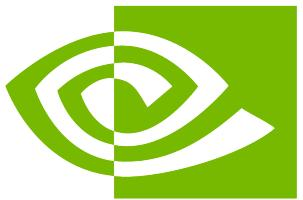
\includegraphics[keepaspectratio,alt={image}]{images/d079ea90faf002ff29d6d955d968923718c19f29218193ce750da21bae99e057.jpg}}

\section{NVIDIA ?}\label{nvidia}

\section{NVIDIA DGX SuperPOD: Next Generation Scalable Infrastructure
for AI Leadership Reference Architecture Featuring NVDIA DGX
GB200}\label{nvidia-dgx-superpod-next-generation-scalable-infrastructure-for-ai-leadership-reference-architecture-featuring-nvdia-dgx-gb200}

Release latest

NVIDIA Corporation

Sep 03, 2025

\section{Reference Architecture}\label{reference-architecture}

1 Abstract 2

2 DGX SuperPOD Architecture 4

3 Key Components of the DGX SuperPOD 5

3.1 NVIDIA DGX GB200 Rack System 5

3.1.1 DGX GB200 Compute Tray 6

3.1.2 NVLink Switch Tray 8

3.1.3 DGX Power Shelves 8

3.2 NVIDIA InfiniBand Technology 8

3.3 NVIDIA Mission Control 9

3.4 Components 9

3.5 Design Requirements . 11

3.5.1 System Design . 11

3.5.2 Compute Fabric 12

3.5.3 Storage Fabric (High Speed Storage) 12

3.5.4 In-Band Management Network 12

3.5.5 Out-of-Band Management Network 12

3.5.6 Storage Requirements 12

3.5.6.1 High-Performance Storage 13

3.5.6.2 User Storage 13

4 Network Fabrics 14

4.1 Multi-node NVLink Fabric (NVL5) 14

4.2 Compute Fabric 15

4.3 Storage and In-band Ethernet Fabric . 18

4.4 Network Segmentation of the Ethernet Fabric 19

4.4.1 Storage Network 20

4.4.2 In-Band Management Network 20

4.4.3 Out-of-Band Management Network 22

4.5 Customer Edge Connectivity 23

5 Storage Architecture 24

6 DGX SuperPOD Software 26

6.1 Run:ai 27

7 Summary 29

8 Notices 30

8.1 Notice 30

8.2 Trademarks 31

8.3 Copyright 31

Document Number RA-11338-001 V01

Publication Date 2025-06-16

\section{Tip}\label{tip}

The NVIDIA DGX SuperPOD: Next Generation Scalable Infrastructure for AI
Factories Reference Architecture Featuring NVIDIA DGX GB200 is also
available as a PDF.

\section{Chapter 1. Abstract}\label{chapter-1.-abstract}

The NVIDIA DGX SuperPOD architecture has been designed to power the
next-generation AI factories with unparalleled performance, scalability,
and innovation that supports all customers in the enterprise, higher
education, research, and the public sector. It is a physical twin of the
main NVIDIA research and development system, meaning the company's
infrastructure software, applications, and support are first tested and
vetted on the same architecture.

\pandocbounded{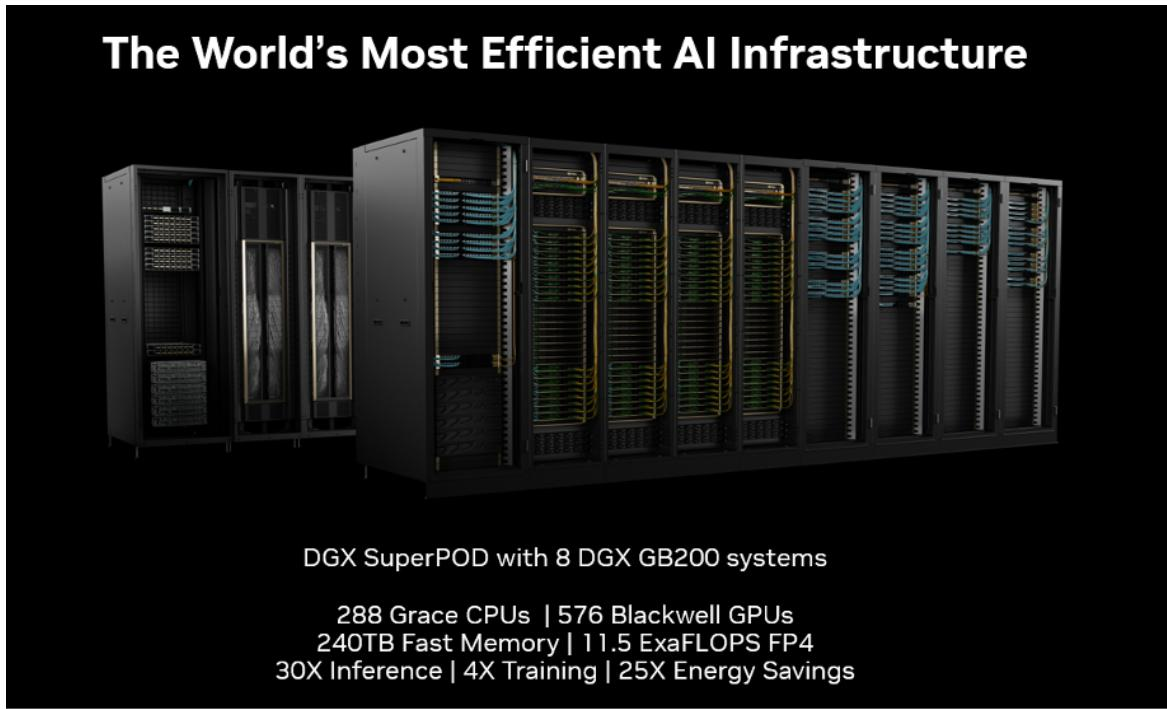
\includegraphics[keepaspectratio,alt={image}]{images/92730ca277f1bd734c5bb9568ee0dc179ac2712a2d70b8c5c6fbbd894119f97e.jpg}}

This DGX SuperPOD Reference Architecture (RA) is based on DGX GB200
systems powered by Grace CPUs and Blackwell GPUs. The RA discusses the
components that define the scalable and modular architecture of DGX
SuperPOD. DGX SuperPOD is built on the concept of scalable units (SU);
each SU contains 8 DGX GB200 systems, which enables rapid deployment of
DGX SuperPOD of anysize. The RA also includes details regarding the SU
design and specifics of InfiniBand, NVLink network, Ethernet fabric
topologies, storage system specifications, recommended rack layouts, and
wiring guidelines.

This RA combines the latest NVIDIA technologies to help companies and
industries develop their own AI factories. To achieve the most
scalability, DGX SuperPOD is powered by several key NVIDIA technologies
and solutions, including:

▶ NVIDIA DGX GB200 systems: Powerful computational building block for AI
and HPC.

▶ NVIDIA NDR (400 Gbps) InfiniBand: High performant, low latency, and
scalable network interconnect.

▶ NVIDIA Spectrum-4 (800 Gbps) Ethernet: High performant, low latency,
and scalable ethernet connectivity for storage.

▶ NVIDIA fifth-generation NVLink® technology: a high-speed interconnect
for CPU and GPU processors in accelerated compute systems to provide
unprecedented performance for most demanding communication patterns.

▶ NVIDIA Mission Control: a unified operations and orchestration
software stack for managing AI factories.

\section{Chapter 2. DGX SuperPOD
Architecture}\label{chapter-2.-dgx-superpod-architecture}

The DGX SuperPOD architecture is a combination of DGX systems,
InfiniBand and Ethernet networking, management nodes, and storage.
Figure 2.1 shows the rack layout of a single SU (Scalable Unit). Each SU
requires a Thermal Design Power (TDP) of 1.2 Megawatts (MW). Generally,
the data center should meet or exceed Uptime Institute Tier 3 design
standards, or alternatively the TIA942-B Rated 3 or EN50600 Availability
Class 3 design standards, including concurrent maintainability and no
single point of failure.

Each DGX GB200 leverages hybrid cooling with both direct liquid cooling
and air cooling to manage the amount of heat produced by each rack.
Given DGX SuperPOD with DGX GB20 is a turnkey AI data center scale
product, NVIDIA has provided datacenter design guidance and fully
integrated operational technology (OT) integration with NVIDIA Mission
Control software stack.

\pandocbounded{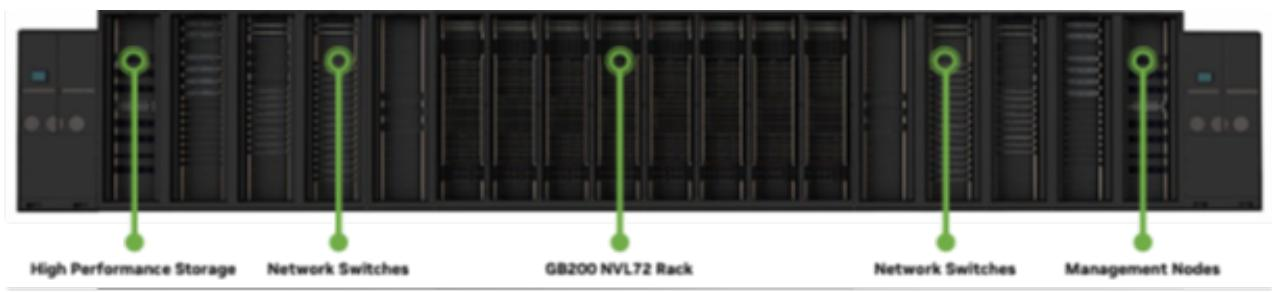
\includegraphics[keepaspectratio,alt={image}]{images/ce4bc0aebe6376661f87290d304fc49f1630c48f8aff62fd1cf1ea79038e7910.jpg}}

Figure 2.1: Complete Rack Layout in One Row

This reference architecture is focused on the design of a single SU (8
DGX GB200 rack systems). DGX SuperPOD can scale to much larger
configurations up to and beyond 128 racks with 9216 GPUs.

Contact your NVIDIA representative for information regarding DGX
SuperPOD solutions of four SUs or more.

\section{Chapter 3. Key Components of the DGX
SuperPOD}\label{chapter-3.-key-components-of-the-dgx-superpod}

The DGX SuperPOD architecture is designed to meet the high demands of AI
factories for the era of reasoning. AI factories require specialized
components like high-performance GPUs and CPUs, advanced networking, and
cooling systems to support the intensive computational needs of AI
workloads. These factories excel at AI reasoning---enabling faster, more
accurate decision-making across industries. And using NVIDIA's
end-to-end accelerated computing platform, they're optimized for energy
efficiency while accelerating AI inference performance, helping
enterprises deploy secure, futureready AI infrastructure.

DGX SuperPOD is the integration of key NVIDIA components, as well as
storage solutions from partners certified to work in a DGX SuperPOD
environment. By leveraging the concept of Scalable Units (SUs, as
defined below in this document), DGX SuperPOD reduces AI factory
deployment times from months to weeks, which in turn reduces
time-to-solution and time-to-market of next generation models and
applications.

DGX SuperPOD is to be deployed on-premises, meaning the customer owns
and manages the hardware. This can be within a customer's data center or
co-located at a commercial data center, but the customer owns the
hardware, the service it provides, and is responsible for their cluster
infrastructure.

The key components of DGX GB200 SuperPOD are shown below, each component
will be discussed in detail:

▶ NVIDIA DGX GB200 NVL72 rack system

▶ NVIDIA InfiniBand

▶ Mission Control software platform

\section{3.1. NVIDIA DGX GB200 Rack
System}\label{nvidia-dgx-gb200-rack-system}

The NVIDIA DGX GB200 system (Figure 3.1) is an AI powerhouse that
enables enterprises to expand the frontiers of business innovation and
optimization. Each DGX GB200 delivers breakthrough AI performance in a
rack-scale, 72 GPU configuration. The NVIDIA Blackwell GPU architecture
provides the latest technologies that brings months of computational
effort down to days and hours, on some of the largest AI/ML workloads.

To accommodate the high compute density per rack and at the same time to
more efficiently use datacenter space, the DGX GB200 rack system employs
a sophisticated hybrid cooling solution to manage the substantial heat
generated by the powerful GPUs and other components. The most
powerintensive components, such as GPUs and CPUs, are liquid cooled.
Other components are air cooled.

NVIDIA's Infrastructure Specialist team can provide end-to-end
assistance for datacenter planning, system deployment, and bring-up
services.

2xManagement top of rack Ethernet switches

4 x Power shelves

10 x Compute Nodes

9 x NVLink switches

8x Compute Nodes

4xPower shelves

Seismic bracing

\pandocbounded{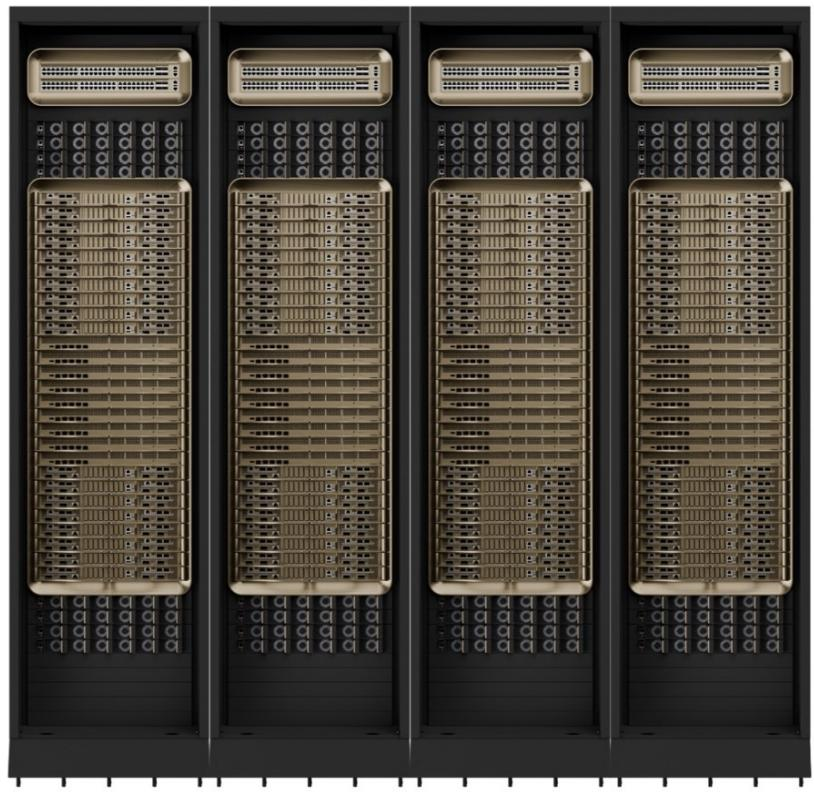
\includegraphics[keepaspectratio,alt={image}]{images/b9a1fb139dbd4a8bfe6a299e128182591b8fcd891ef7f3139cd3b43ce105ef11.jpg}}

Figure 3.1: DGX GB200 (4 racks are shown here)

\section{3.1.1. DGX GB200 Compute Tray}\label{dgx-gb200-compute-tray}

The compute nodes for DGX GB200 rack system are using the 72x1 NVLink
topology, which contains 72 GPUs in a single NVLink domain. There are 18
compute nodes (AKA trays) in a DGX GB200 rack system. Each compute tray
contains two GB200 Superchips, and each Superchip has two B200 GPUs and
one Grace CPU. A coherent chip-to-chip interconnect link, called
NVLink-C2C, bridges the two Superchips and enables them to act as a
single logical unit for a single OS instance to operate.

The compute tray integrates four ConnectX-7 (CX-7) NICs to support
InfiniBand NDR (400Gbps) connectivity for the cross racks Compute
network, and two BlueFiled-3 (BF3) NICs to support 2x200Gbps
connectivity for the In-band Management and Storage networks. All
network ports are located at the front-side of the rack, intentionally
for the cold aisle.

Each compute tray also provides a total of 4x 3.84TB E1.S NVMe as RAID0
for local storage and 1x 1.92TB M.2 NVMe for the OS image.

Figure 3.2 and Figure 3.3 show the front and rear of a DGX GB200 compute
tray respectively.

Figure 3.4 shows the block diagram of the GB200 compute tray with two
GB200 Superchips, each chip combines two NVIDIA B200 Tensor Core GPUs
and one NVIDIA Grace CPU, connected over a 900GB/s ultra-low-power
NVLink-C2C interconnect.

\pandocbounded{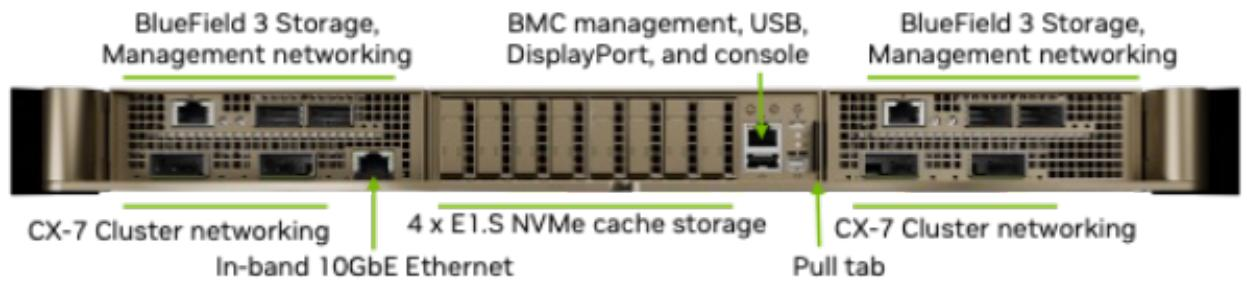
\includegraphics[keepaspectratio,alt={image}]{images/b74e264be2372395ac2b69739415cb7f86f29696bf19f4957ded047b8767f2a4.jpg}}

Figure 3.2: GB200 Compute Tray Front

\pandocbounded{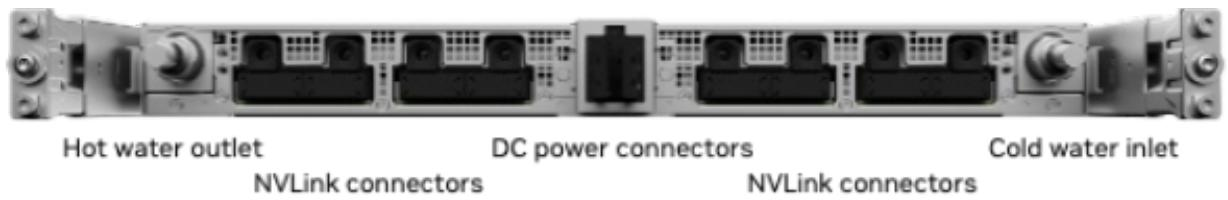
\includegraphics[keepaspectratio,alt={image}]{images/4acadea3feeb1e856a4462eb4a46afc4d4aa548849067a7acd7c09ca4b27c5cc.jpg}}

Figure 3.3: GB200 Compute Tray Rear

\pandocbounded{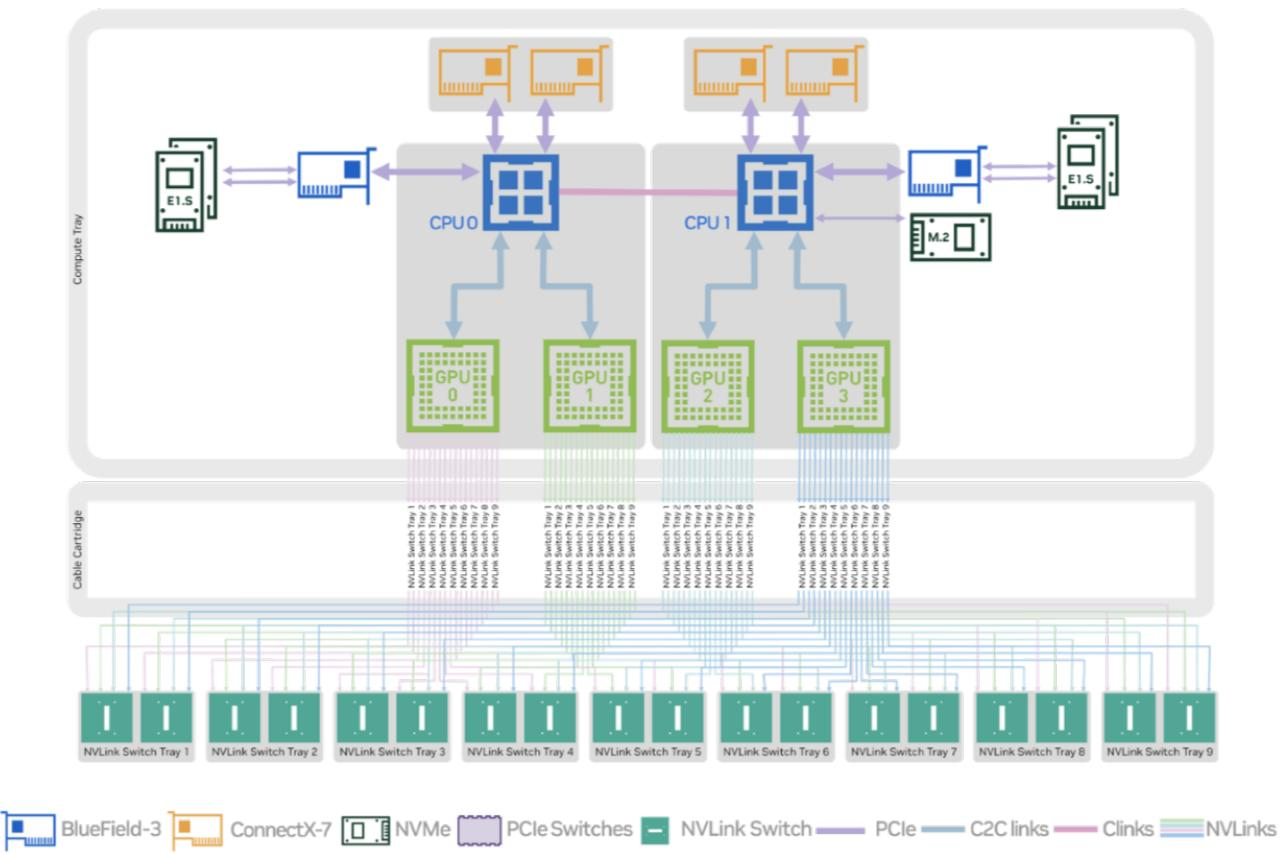
\includegraphics[keepaspectratio,alt={image}]{images/094a6ee21126b9e9415800ccb7e6af64479888014f3ae4878f73b3a8d5691670.jpg}}

Figure 3.4: GB200 Compute Tray Block Diagram

\section{3.1.2. NVLink Switch Tray}\label{nvlink-switch-tray}

Each DGX GB200 NVL72system rack also features nine NVLink switches (AKA
NVLink switch tray). All NVLink interconnections are done through the
rear-side, blind-mate connectors to the cable cartridges within the
rack. Each switch tray features two COMe RJ45 ports for NVOS and one BMC
module for out-of-band management with one RJ45 port. Figure 3.5
showcases the front design of a NVLink Switch Tray.

\pandocbounded{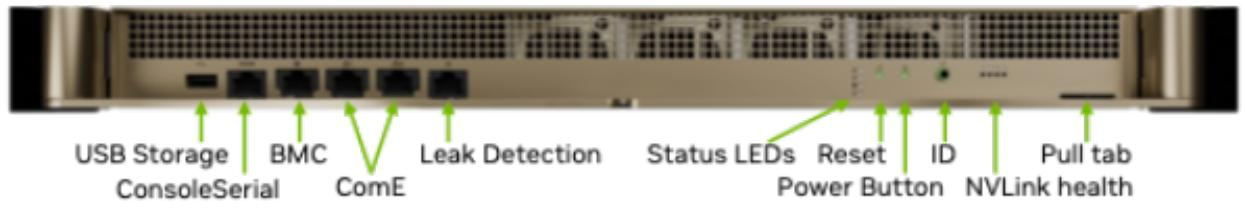
\includegraphics[keepaspectratio,alt={image}]{images/e0dbc324d6ae62d8592a8c29550fdafaf5263e32fd5088d995092fa53d84452c.jpg}}

Figure 3.5: GB200 Compute Tray Block Diagram

\section{3.1.3. DGX Power Shelves}\label{dgx-power-shelves}

The power shelf used for DGX DGX GB200 SuperPOD has six 5.5kW PSUs
configured as N redundancy and can deliver up to 33kW of power. There
are eight total power shelves in a single DGX GB200 NVL72 rack system.
At the rear of the power shelf is a set of RJ45 ports used for power
brake and current sharing feature. The power shelves are daisy chained
to each other using these RJ45 ports. At the front of the power shelf is
the BMC port. Figure 3.6 shows the front of the power shelf.

\pandocbounded{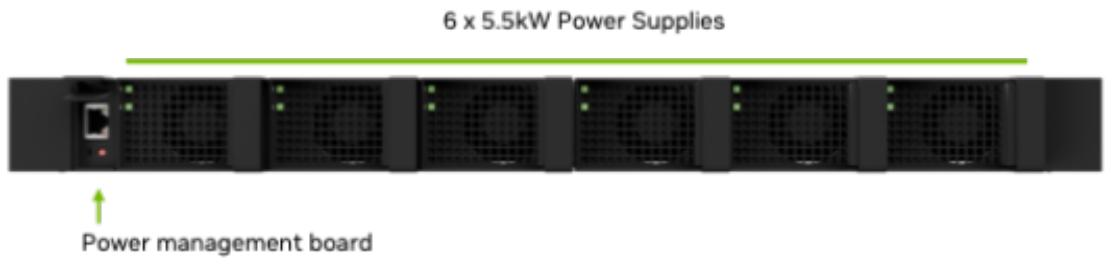
\includegraphics[keepaspectratio,alt={image}]{images/3e3a679097d071daaa08a6182df18534570b74e3078ed3439420930e0fd71407.jpg}}

Figure 3.6: Power Shelf

\section{3.2. NVIDIA InfiniBand
Technology}\label{nvidia-infiniband-technology}

InfiniBand is a high-performance, low latency, RDMA capable networking
technology, proven over 20 years in the harshest compute environments to
provide the best inter-node network performance. InfiniBand continues to
evolve and lead data center network performance.

The latest generation InfiniBand, NDR, has a peak speed of 400 Gbps per
direction with an extremely low port-to-port latency. It is backwards
compatible with the previous generations of InfiniBand specifications.
InfiniBand is more than just peak bandwidth and low latency. It provides
additional features to optimize performance including adaptive routing
(AR), collective communication with SHARPTM, dynamic network healing
with SHIELDTM, and supports several network topologies including
fat-tree, Dragonfly, and multi-dimensional Torus to build the largest
network fabrics and computer systems possible.

\section{3.3. NVIDIA Mission Control}\label{nvidia-mission-control}

The DGX GB200 SuperPOD Reference Architecture represents the best
practices for building highperformance AI factories. There is
flexibility in how these systems can be presented to customers and
users. NVIDIA Mission Control software is used to manage all DGX GB200
SuperPOD deployments.

NVIDIA Mission Control is a sophisticated full-stack software solution.
As an essential part of the DGX SuperPOD experience, it optimizes
developer workload performance and resiliency, ensures continuous uptime
with automated failure handling, and provides unified cluster-scale
telemetry and manageability. Key features include full-stack resiliency,
predictive maintenance, unified error reporting, data center
optimizations, cluster health checks, and automated node management.

Mission Control software incorporates the same technology that NVIDIA
uses to manage thousands of systems for our ad-winning data scientists
and provides an immediate path to a TOP500 supercomputer for
organizations that need the best of the best.

DGX SuperPOD is to be deployed on-premises, meaning the customer owns
and manages the hardware. This can be within a customer's data center or
co-located at a commercial data center, but the customer owns the
hardware, the service it provides, and is responsible for their cluster
infrastructure as well as providing the building management system for
integration.

\section{3.4. Components}\label{components}

The hardware components of DGX SuperPOD are described in Table 3.1. The
software components are shown in Table 3.2.

Table 3.1: DGX SuperPOD hardware components by NVIDIA

{\def\LTcaptype{none} % do not increment counter
\begin{longtable}[]{@{}|l|l|l|@{}}
\toprule\noalign{}
\endhead
\bottomrule\noalign{}
\endlastfoot
\hline
Component & Technology & Description \\
\hline
8x Compute Racks & NVIDIA DGX GB200 NVL72 & The world\textquotesingle s
premier rack-scale, purpose-built AI systems featuring NVIDIA
Grace-Blackwell GB200 modules. GB200 Superchips. NVL72 scale-out GPU
interconnect and integrated NVLink switch trays. \\
\hline
NVLink Fabric & NVIDIA NVLink 5 & NVLink Switches supports fast, direct
memory access between GPUs on the same compute rack. \\
\hline
Compute Fabric & NVIDIA Quantum QM9700 InfiniBand switches &
Rail-optimized, non-blocking, full fat-tree network with eight NDR400
connections per system for cross rack GPU communications. \\
\hline
Storage and In-band Management Fabric & NVIDIA Spectrum 4 SN5600
Ethernet switches & The fabric is optimized to match peak performance of
the configured storage array, built with 64 port 800 Gbps Ethernet
switch providing high port density with high performance. \\
\hline
InfiniBand management & NVIDIA Unified Fabric Manager Appliance,
Enterprise Edition & NVIDIA UFM combines enhanced, real-time network
telemetry with AI powered cyber intelligence and analytics to manage
scale-out InfiniBand data centers \\
\hline
NVLink Management & NVIDIA Network Manager eXperience (NMX) & NVIDIA NMX
manages, operates the NVLink switches and provides real-time network
telemetry to manage all NVLink infrastructure \\
\hline
Out-of-band (OOB) management network & NVIDIA SN2201 switch & 48 x 1
Gbps Ethernet switch leveraging copper ports to minimize complexity \\
\hline
\end{longtable}
}

Table 3.2: DGX SuperPOD software components

{\def\LTcaptype{none} % do not increment counter
\begin{longtable}[]{@{}|l|l|l|@{}}
\toprule\noalign{}
\endhead
\bottomrule\noalign{}
\endlastfoot
\hline
\multicolumn{2}{@{}l}{%
Component} & Description \\
\hline
Mission Software & Control & NVIDIA Mission Control software delivers a
full stack data center solution engineered for NVIDIA DGX SuperPOD with
DGX GB200 or DGX B200 infrastructure deployments. It integrates
essential management and operational capabilities into a unified
platform, thereby providing enterprise customers with simplified control
over their NVIDIA DGX SuperPOD infrastructure deployments at scale.
NVIDIA Mission Control also leverages NVIDIA Run;ai functionality,
providing seamless workload orchestration. \\
\hline
NVIDIA AI Enterprise & Enterprise & NVIDIA AI Enterprise is an
end-to-end, cloud-native software platform that accelerates data science
pipelines and streamlines development and deployment of production-grade
LLMs and other generative AI applications. \\
\hline
Magnum IO & IO & Enables increased performance for AI and HPC \\
\hline
NVIDIA NGC & NGC & The NGC catalog provides a collection of
GPU-optimized containers for AI and HPC \\
\hline
Slurm & Slurm & A classic workload manager used to manage complex
workloads in a multi-node, batch-style, compute environment \\
\hline
\end{longtable}
}

\section{3.5. Design Requirements}\label{design-requirements}

DGX SuperPOD is designed to minimize system bottlenecks throughout the
tightly coupled configuration to provide the best performance and
application scalability. Each subsystem has been thoughtfully designed
to meet this goal. In addition, the overall design remains flexible so
that SuperPOD can be tailored to better integrate into existing data
centers.

\section{3.5.1. System Design}\label{system-design}

DGX SuperPOD is optimized for a customers' particular workload of
multi-node AI and HPC applications:

▶ A modular architecture based on Scalable Units (SUs) of 8 DGX GB200
systems.NVL72 rack systems.

▶ A fully tested system scales to two SUs, but larger deployments can be
built based on customer requirements

▶ Rack-A fully tested system scales for a single SU, seamlessly.

▶ level integrated design which allows rapid installation and deployment
of liquid cooled, high density compute racks.

▶ Storage partner equipment that has been certified to work in DGX
SuperPOD environment.

▶ Storage partner equipment that has been certified to work in DGX
SuperPOD environments.

▶ Full system support---including compute, storage, network, and
software---is provided by NVIDIA Enterprise Support (NVEX).

\section{3.5.2. Compute Fabric}\label{compute-fabric}

▶ The compute fabric is rail-optimized to the top layer of the fabric.

▶ The compute fabric is a balanced, full-fat tree.

▶ The compute fabric is designed with current state-of-the-art, top
performing, high-performance, low-latency network switches, and supports
future generation of networking hardware.

▶ Managed NDR switches are used throughout the design to provide better
management of the fabric.

▶ The fabric is designed to support the latest SHARPv3 features.

\section{3.5.3. Storage Fabric (High Speed
Storage)}\label{storage-fabric-high-speed-storage}

The storage fabric provides high bandwidth to shared storage. It also
has the following characteristics:

▶ It is independent of the compute fabric to maximize performance of
both storage and application performance.

▶ Provides single-node line-rate of 2x 200Gbps to each DGX GB200 compute
tray.

▶ Storage is provided over RDMA over Converged Ethernet to provide
maximum performance and minimize CPU overhead.

▶ User-accessible management nodes provide access to shared storage.

\section{3.5.4. In-Band Management
Network}\label{in-band-management-network}

▶ The in-band management network fabric is Ethernet-based and is used
for node provisioning, data movement, Internet access, and other
services that must be accessible by the users.

▶ The in-band management network connections for compute and management
nodes operate at 200 Gbps and are bonded for resiliency.

\section{3.5.5. Out-of-Band Management
Network}\label{out-of-band-management-network}

The OOB management network connects all the baseboard management
controllers (BMC), BlueField baseboard management controllers, NVSwitch
Management Interfaces (COMe), as well as other devices that should be
physically isolated from system users.

\section{3.5.6. Storage Requirements}\label{storage-requirements}

The DGX SuperPOD compute architecture must be paired with a
high-performance, balanced, storage system to maximize overall system
performance. DGX SuperPOD is designed to use two separate storage
systems, high-performance storage (HPS) and user storage, optimized for
key operations of throughput, parallel I/O, as well as higher IOPS and
metadata workloads.

\section{3.5.6.1 High-Performance
Storage}\label{high-performance-storage}

High-Performance Storage is provided via RDMA over Converged Ethernet v2
(RoCEv2) connected storage from a DGX SuperPOD certified storage
partner, and is engineered and tested with the following attributes in
mind:

▶ High-performance, resilient, POSIX-style file system optimized for
multi-threaded read and write operations across multiple nodes.

▶ Certified for Grace-based systems.

▶ Native RoCE support.

▶ Local system RAM for transparent caching of data.

▶ Leverage local flash device transparently for read and write caching.

The specific storage fabric topology, capacity, and components are
determined by the DGX SuperPOD certified storage partner as part of the
DGX SuperPOD design process.

\section{3.5.6.2 User Storage}\label{user-storage}

User Storage differs from High-Performance storage in that it exposes an
NFS share on the in-band management fabric for multiple uses. It is
typically used for ``home directory'' type usage (especially with
clusters deployed with SLURM), administrative scratch space, and shared
storage as needed by DGX SuperPOD components in a High Availability
configuration (e.g., Mission Control), the requirement for log files
collection, and system configuration files.

With that in mind, User Storage has the following requirements:

▶ Designed for high metadata performance, IOPS, and key enterprise
features such as log collection, data capacity. This is different than
the HPS, which is optimized for parallel I/O and large capacity.

▶ Communicate over Ethernet, using NFS.

▶ 100GbE DR1 Connectivity.

User storage in a DGX SuperPOD is often satisfied with existing NFS
servers already deployed, such that a new export is created and made
accessible to the DGX SuperPOD's in-band management network. User
Storage is therefore not described in detail in this DGX SuperPOD
reference architecture.

\section{Chapter 4. Network Fabrics}\label{chapter-4.-network-fabrics}

Building systems by SU provides the most efficient designs. However, if
a different node count is required due to budgetary constraints, data
center constraints, or other needs, the fabric should be designed to
support the full SU, including leaf switches and leaf-spine cables, and
leave the portion of the fabric unused where these nodes would be
located. This will ensure optimal traffic routing and ensure that
performance is consistent across all portions of the fabric.

DGX SuperPOD configurations utilize five network fabrics:

▶ NVLink 5

▶ Compute Fabric

▶ Storage Fabric

▶ In-Band Management Network

▶ Out-of-Band Management Network

These network segments are carried by four different physical fabrics:

▶ Multi-node NVLink Fabric (MN-NVL)

▶ Compute InfiniBand Fabric

▶ Storage and In-band Ethernet Fabric

▶ Out-of-Band network

▶ Each of these fabrics are discussed in this section.

\section{4.1. Multi-node NVLink Fabric
(NVL5)}\label{multi-node-nvlink-fabric-nvl5}

Each DGX GB200 rack is built with 18 compute trays and 9 NVLink switch
trays. Each NVLink switch tray is equipped with 2 NVLink switch chips
and are responsible for the full-mesh connectivity between all 72 GPUs
within the same DGX GB200 rack. Each B200 GPU features 18 NVL5 links and
has one dedicated NVL5 link connectivity to each one of the 18 switch
chips, delivering a total bandwidth of 1.8 TB/s low latency bandwidth.

\section{Note}\label{note}

Each network is detailed in this section.

Figure 4.1 shows the ports on the back of the DGX B200 CPU tray and the
connectivity provided. The compute fabric ports in the middle use a
two-port transceiver to access all eight GPUs. Each pair

of in-band management and storage ports provide parallel pathways into
the DGX B200 ystem for increased performance. The OOB port is used for
BMC access. (The LAN port next to the BMC port is not used in DGX
SuperPOD configurations.)

\pandocbounded{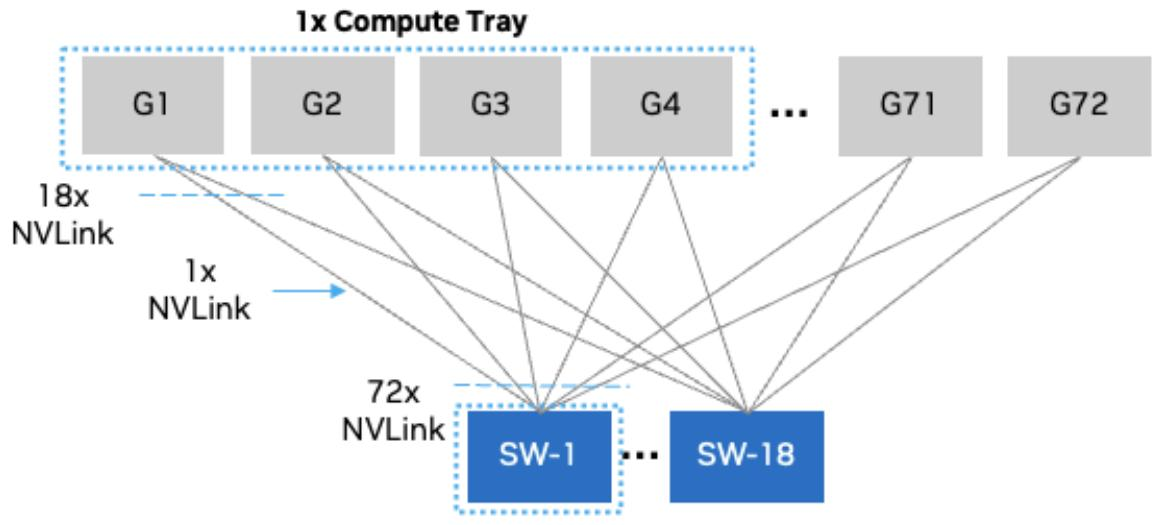
\includegraphics[keepaspectratio,alt={image}]{images/c36aabcd75c5c02a63f5d016185acb16e19398b4fa3f720e652b23814b355c7d.jpg}}

Figure 4.1: Multi-node NVLink Topology

\section{4.2. Compute Fabric}\label{compute-fabric-1}

Figure 4.2 shows the compute fabric layout for the full GB200 SuperPOD
Scalable Unit (8 DGX GB200 systems). Each compute rack is rail-aligned.
Traffic per rail of each compute tray is always one hop away from other
compute trays in the same Scalable Unit. Traffic between different
compute racks, or between different rails, traverses the spine layer.

For designs larger than one SU, we provide spine-leaf-group (SLG) based
scalable design with scalability for up to and including 16 SUs. Each SU
contains 4 SLGs to match with the number of IB rails (which equals the
number of GPUs per compute tray). There are 8 leaf switches (one for
each compute rack) and 6 spine switches in each SLG -- allowing a fully
non-blocking fat tree topology for each SU to be attached to 6 core
groups. The details of this design for scale-out is presented in Figure
4.3. Table 4.1 shows an outline for the switches required for scale out
build of DGX SuperPOD.

Table 4.1: Larger SuperPOD component counts

{\def\LTcaptype{none} % do not increment counter
\begin{longtable}[]{@{}lllllllll@{}}
\toprule\noalign{}
\endhead
\bottomrule\noalign{}
\endlastfoot
\multirow{2}{*}{\# GPUs} & \multirow{2}{*}{\# SUs} & \multirow{2}{*}{\#
Core Group} & \multirow{2}{*}{Switch per Core Group} &
\multirow{2}{*}{Core Switch} & \multicolumn{2}{l}{%
IB Leaf Switch} & \multicolumn{2}{l@{}}{%
IB Spine Switch} \\
& & & & & Per SU & Total & Per SU & Total \\
1152 & 2 & 6 & 3 & 18 & 32 & 64 & 24 & 48 \\
2304 & 4 & 6 & 6 & 36 & 32 & 128 & 24 & 96 \\
4608 & 8 & 6 & 12 & 72 & 32 & 256 & 24 & 192 \\
9216 & 16 & 6 & 24 & 144 & 32 & 512 & 24 & 384 \\
\end{longtable}
}

\pandocbounded{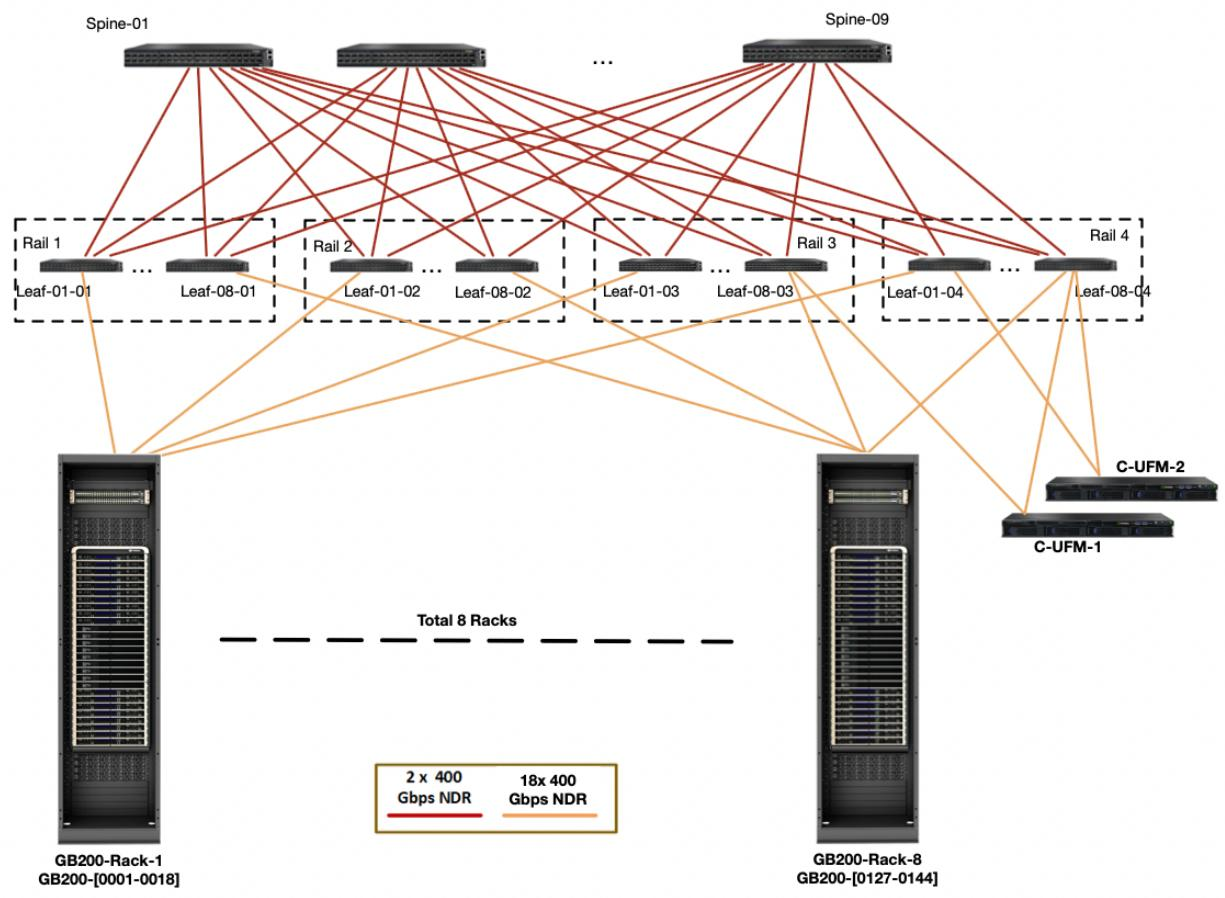
\includegraphics[keepaspectratio,alt={image}]{images/ba8e6a5cae7de2117acbc1e6db2edce6e79f1c8b4119ed3e78fe81bdc19a6857.jpg}}

Figure 4.2: Compute fabric for full 576 GPUs DGX SuperPOD

\pandocbounded{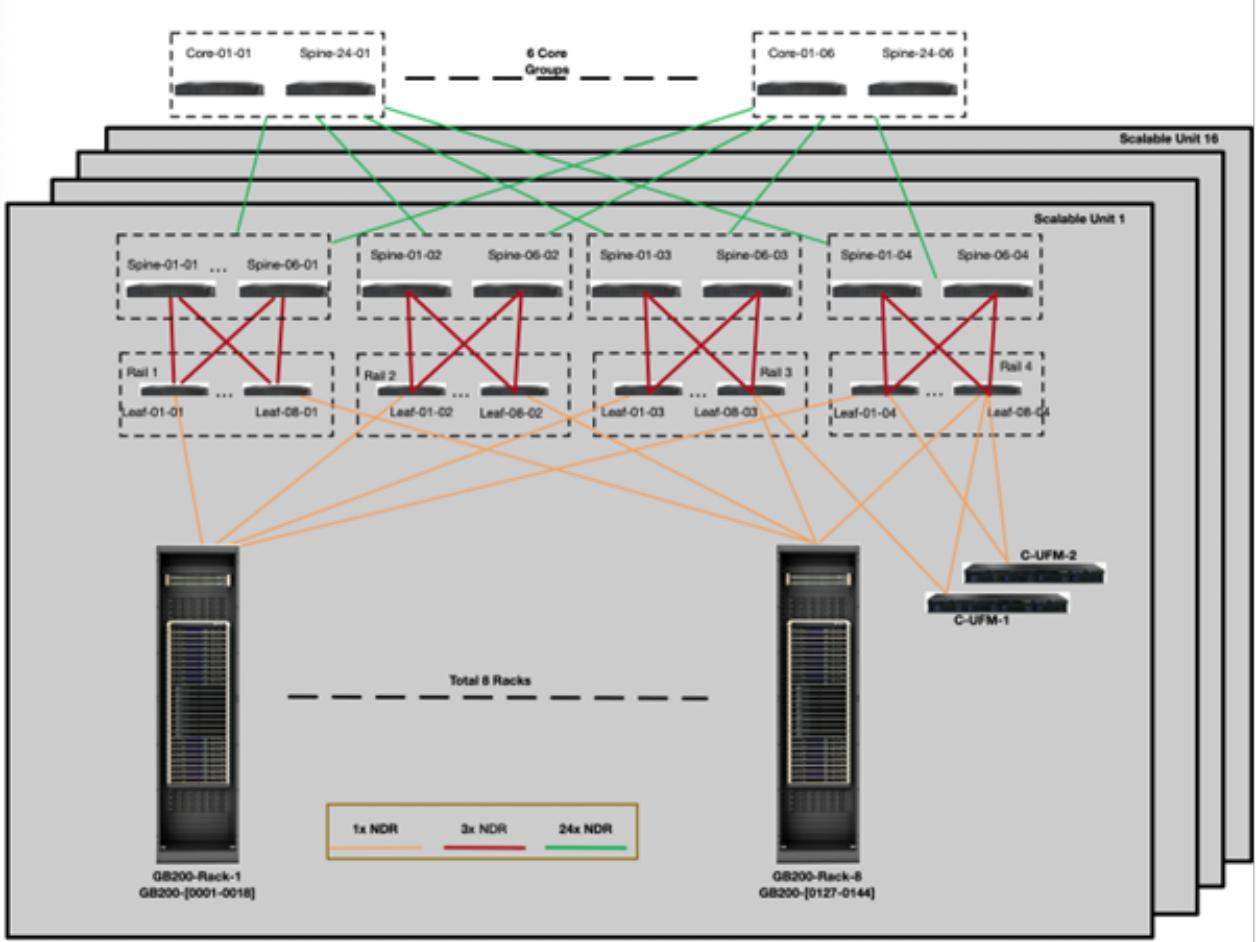
\includegraphics[keepaspectratio,alt={image}]{images/9a6b8aaa195a111ff65bf1fc4803d34f7929436dfd889100b89024b41ec295c5.jpg}}

Figure 4.3: Compute Fabric for Scale Out of up to 16 SUs

\section{4.3. Storage and In-band Ethernet
Fabric}\label{storage-and-in-band-ethernet-fabric}

With DGX GB200, we introduced a new generation of ethernet-based fabric
for storage and in-band network to enhance cost-efficiency while
maintaining the high level of performance required by the storage
network in a large-scale AI training cluster.

The storage and in-band fabric use SN5600 switches and SN2201 switches
shown in Figure 4.4 and Figure 4.5 respectively.

\pandocbounded{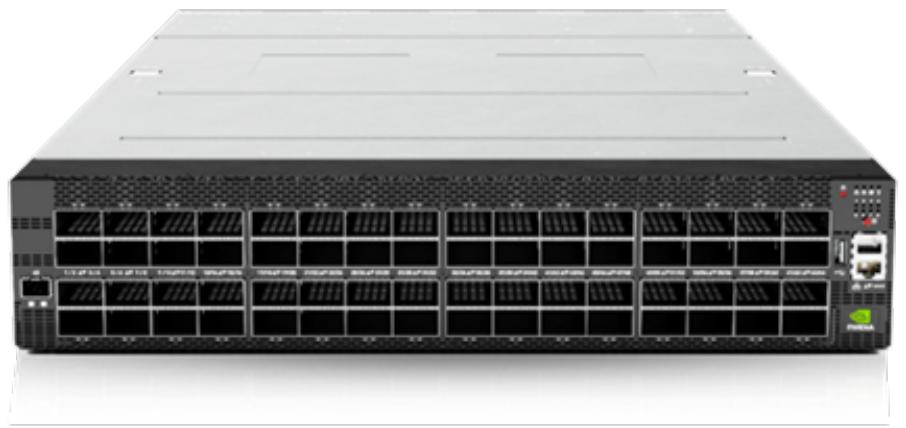
\includegraphics[keepaspectratio,alt={image}]{images/115024adf61771de76194b12efd1a1d39c17afabb9ed276ab37ae27d25839df7.jpg}}

Figure 4.4: SN5600 Switch

\pandocbounded{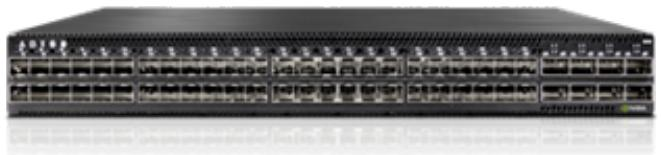
\includegraphics[keepaspectratio,alt={image}]{images/973c8f888305e799c625da10c89d3baa24795d32c8aab28dcb78be9c4f98d5d2.jpg}}

Figure 4.5: SN2201 Switch

Figure 4.6 shows the physical layout of a single SU. Figure 12 shows the
physical layout of a single SU. Each SU features two SN5600 switches as
the aggregation layer or spine layer for the physical network. Here --
all the leaf level switches facing DGX, Storage, and the out-of-band
connection are aggregated on these pair of switches. On the leaf layer,
DGX compute trays are connected at 4x 200GbE on their BlueField 3 DPUs.
One additional pair of SN5600 switches serves as the ingestion point for
Storage Appliances and control plane nodes. One additional pair of
SN2201 switches are to connect all legacy devices requiring RJ45
connections or QSFP based uplink connectivity.

To achieve desired scale-out to up to and including 16 SUs, a third
layer of switches -- known as super spine -- are added. Figure 4.7 shows
the scale-out design for SuperPOD. Similar to the compute fabric, each
SU in the SuperPOD can be implemented incrementally -- given the super
spine layer is built to support the maximum number of spine switches in
the SuperPOD. The super spine is designed with 2 groups. Each Spine is
expected to have 28x 800GbE connection uplinks to maintain non-blocking
characteristics for the disaggregated storage design in the scalable
SuperPOD reference architecture.

Figure 4.7 shows this design for scale out and Table 4.2 summarize the
required number of switches for example size of SUs.

\pandocbounded{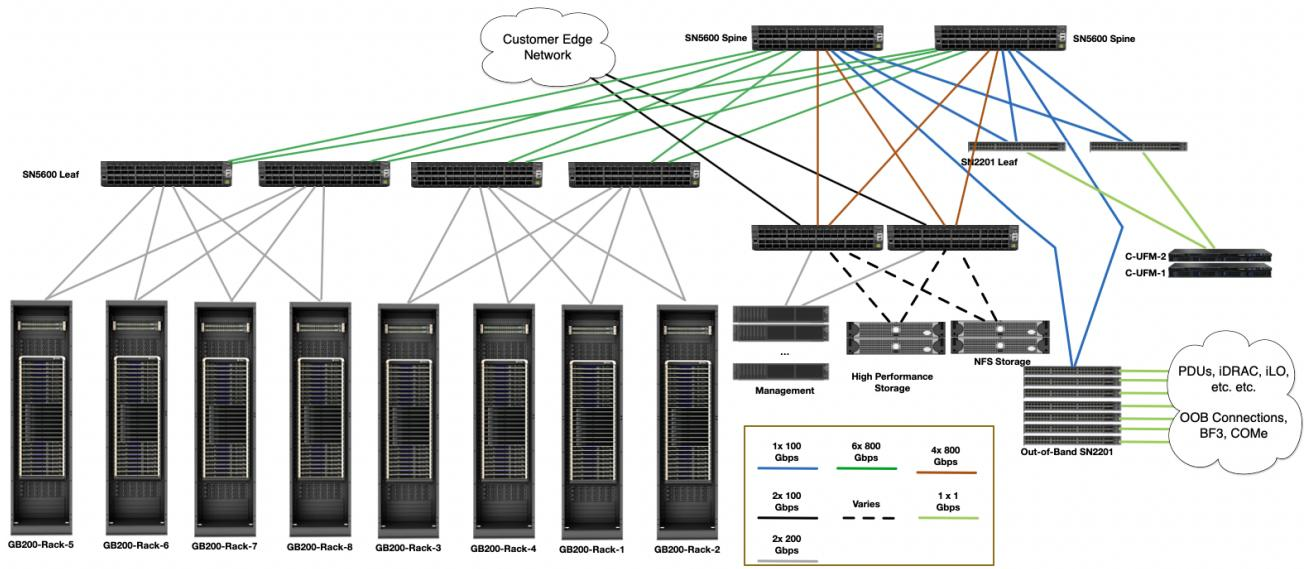
\includegraphics[keepaspectratio,alt={image}]{images/b60361e214c964a5d0ab49cee25bfa69bb8a598cf3e29770486bb583d907fec0.jpg}}

Figure 4.6: Storage and In-band Ethernet fabric logical design

Table 4.2: Spine and Super Spine Switch Requirements for Scale Out

{\def\LTcaptype{none} % do not increment counter
\begin{longtable}[]{@{}lllllllll@{}}
\toprule\noalign{}
\endhead
\bottomrule\noalign{}
\endlastfoot
\multirow{2}{*}{\# GPUs} & \multirow{2}{*}{\# SUs} & \multirow{2}{*}{\#
Super Spine Groups} & \multirow{2}{*}{Super Spines per Group} &
\multirow{2}{*}{\# Super Spine Switches} & \multicolumn{2}{l}{%
\# Spine Switches} & \multicolumn{2}{l@{}}{%
IB Spine Switch} \\
& & & & & 4 & Total & Per SU & Total \\
2304 & 4 & 2 & 2 & 4 & 8 & 64 & 24 & 48 \\
4608 & 8 & 2 & 4 & 8 & 16 & 128 & 24 & 96 \\
9216 & 16 & 2 & 7 & 14 & 32 & 256 & 24 & 192 \\
9216 & 16 & 6 & 24 & 144 & 32 & 512 & 24 & 384 \\
\end{longtable}
}

\section{4.4. Network Segmentation of the Ethernet
Fabric}\label{network-segmentation-of-the-ethernet-fabric}

The ethernet fabric is segmented into these segments on the SuperPOD:

▶ Storage Network

▶ In-band Network

▶ Out-of-Band Management Network

In the following, we introduce these networks in detail.

\pandocbounded{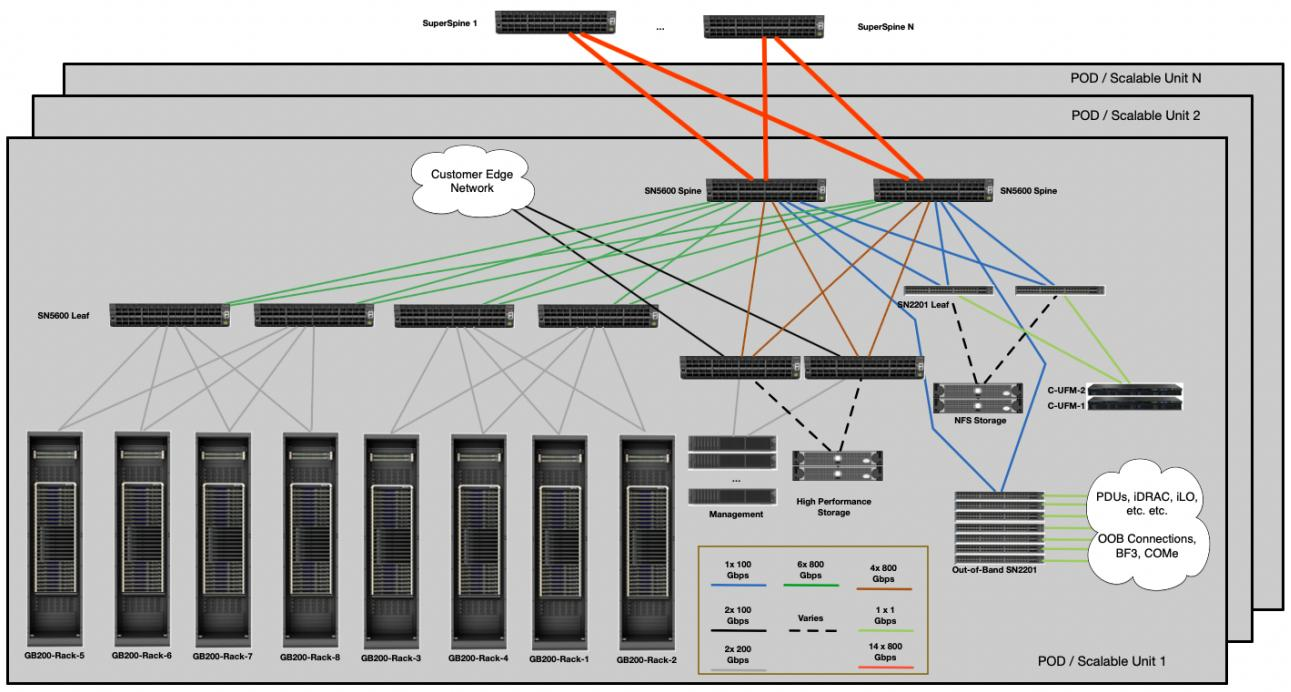
\includegraphics[keepaspectratio,alt={image}]{images/20a49f6c57780d006eab82ca76eddeabbd89be69cdb9b247d3e3df1ac2dac3ef.jpg}}

Figure 4.7: Storage and In-band Ethernet fabric scale out

\section{4.4.1. Storage Network}\label{storage-network}

The storage network embodies the performance for the high-speed storage
while keeping the support for high availability. To achieve this, 2 out
of the 4 available ports on each BlueField-3 DPU are dedicated for
storage access.

The physical ethernet fabric carries a dedicated VXLAN with termination
points on the leaf switches for the DGX nodes' storage NIC ends on each
SN5600 Leaf switches. In addition, one pair of SN5600 leaf in each SU
provides the connectivity to the storage appliances. RoCE is a basic
requirement for the storage appliances, which benefits from advanced
fabric management features, such as congestion control and AR (Adaptive
Routing), provides lower latency while maintaining the high bandwidth
requirement.

Each scalable unit is designed to carry 16x 800Gbps non-blocking
bandwidth to the storage appliances. On the DGX node side, each scalable
unit carries a slightly blocking fabric with a blocking factor of 5:3.
Figure 4.8 shows the logical view of the storage fabric.

\section{4.4.2. In-Band Management
Network}\label{in-band-management-network-1}

The in-band management network provides several key functions:

▶ Connects all the services that manage the cluster.

▶ Enables access to the lower-speed, NFS tier of storage.

▶ Provides uplink (border) connectivity for the in-cluster services such
as Mission Control, Base Command Manager, Slurm, and Kubernetes to other
services outside of the cluster such as the NGC registry, code
repositories, and data sources.

▶ Provides end user access to the Slurm head nodes and Kubernetes
services.

\pandocbounded{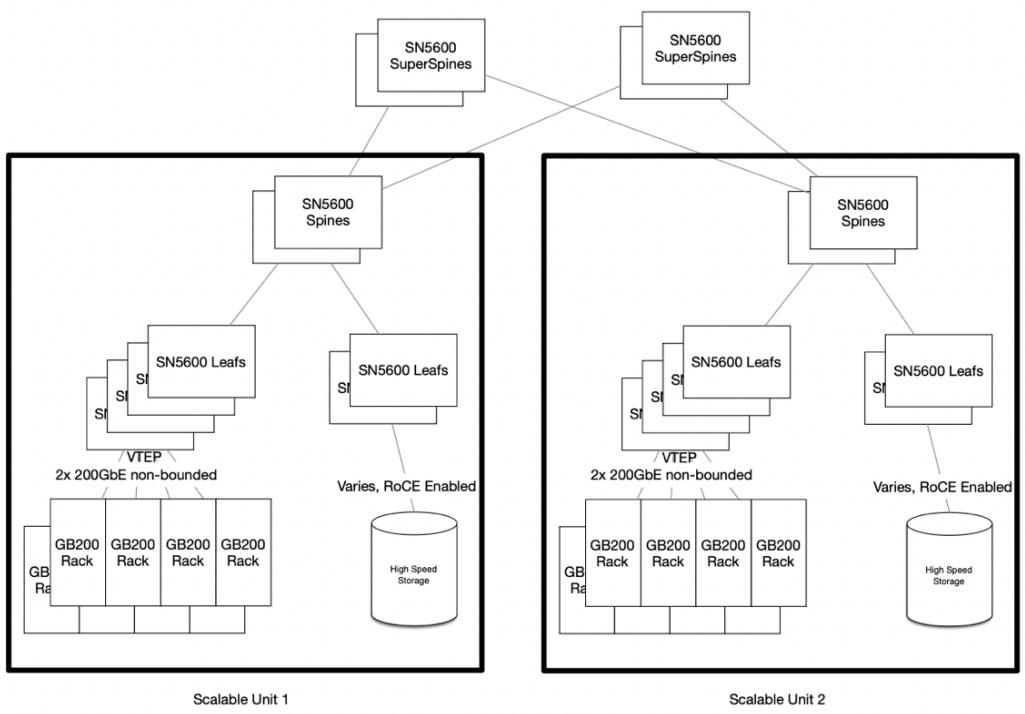
\includegraphics[keepaspectratio,alt={image}]{images/e5a75abc83f4788ce925ad7d0656c0f91e2b0ef7232a4d69f1f05162e8d4dd76.jpg}}

Figure 4.8: Storage Fabric Underlay Network

\pandocbounded{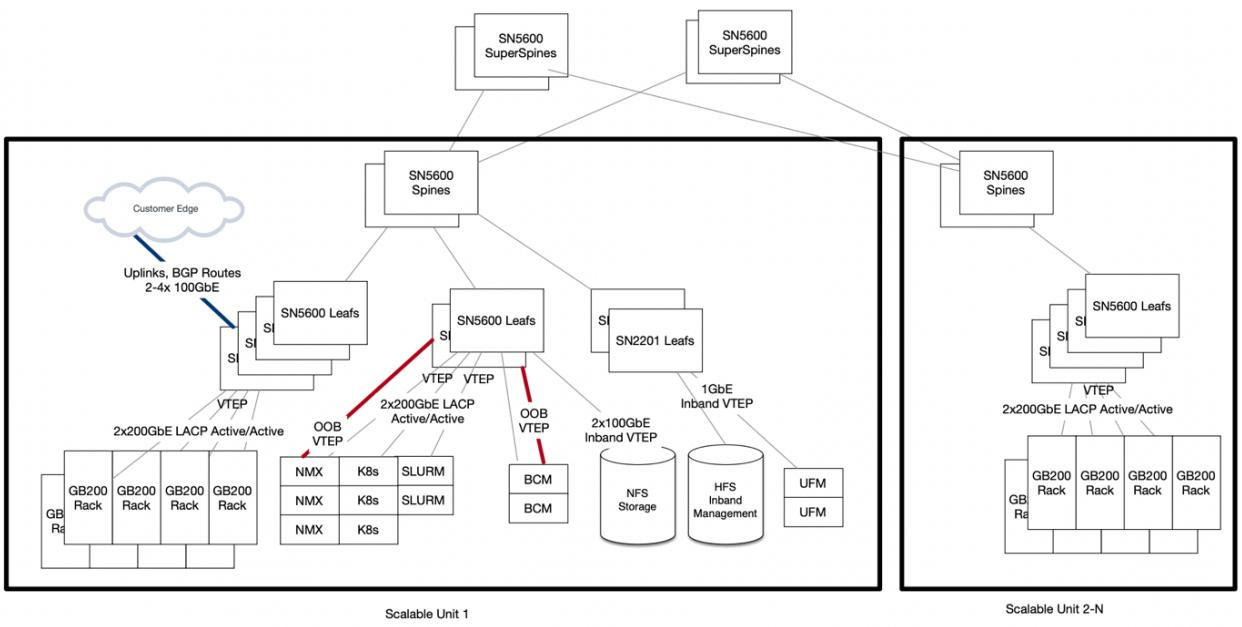
\includegraphics[keepaspectratio,alt={image}]{images/04a8b2685e679efebbd792e10599982182fd53669b20a48a20e5dc341c4b1935.jpg}}

Figure 4.9: In-band Fabric Underlay Network

The in-band network itself is split into 3 different segments:

▶ A dedicated VTEP for uplink, the default hand over to customer edge is
based on BGP peering and providing routes from in-band (and leaked
routes from OOB) to customers' edge.

▶ Customer is also expected to provide link to the building management
system network (BMS) as part of their edge connectivity.

▶ A dedicated VTEP for out-of-band network for the network management
devices (NMX-Manager) and for BCM to access the telemetry and perform
management functions to the OOB devices.

▶ The in-band VTEP, which carries the network for user access,
home-directory storage access via NFS, service delivery, and general
control traffic.

\section{4.4.3. Out-of-Band Management
Network}\label{out-of-band-management-network-1}

Figure 4.10 shows the OOB Ethernet fabric. It connects the management
ports of all devices including DGX GB200 compute trays, switch trays,
and management servers, storage, networking gear, rack PDUs, and all
other devices. These are separated onto their own network. There is no
use-case where a non-privileged user needs direct access to these ports
and are secured using logical network separation.

The OOB network carries all IPMI related control traffic and serves as
the network for fabric management of the compute InfiniBand fabric and
compute NVLink fabric.

The OOB network is physically rolled up into the aggregation layer
(spine layer) of each SU as a dedicated VXLAN. The OOB management
network use SN2201 switches, shown in Figure 4.11

\pandocbounded{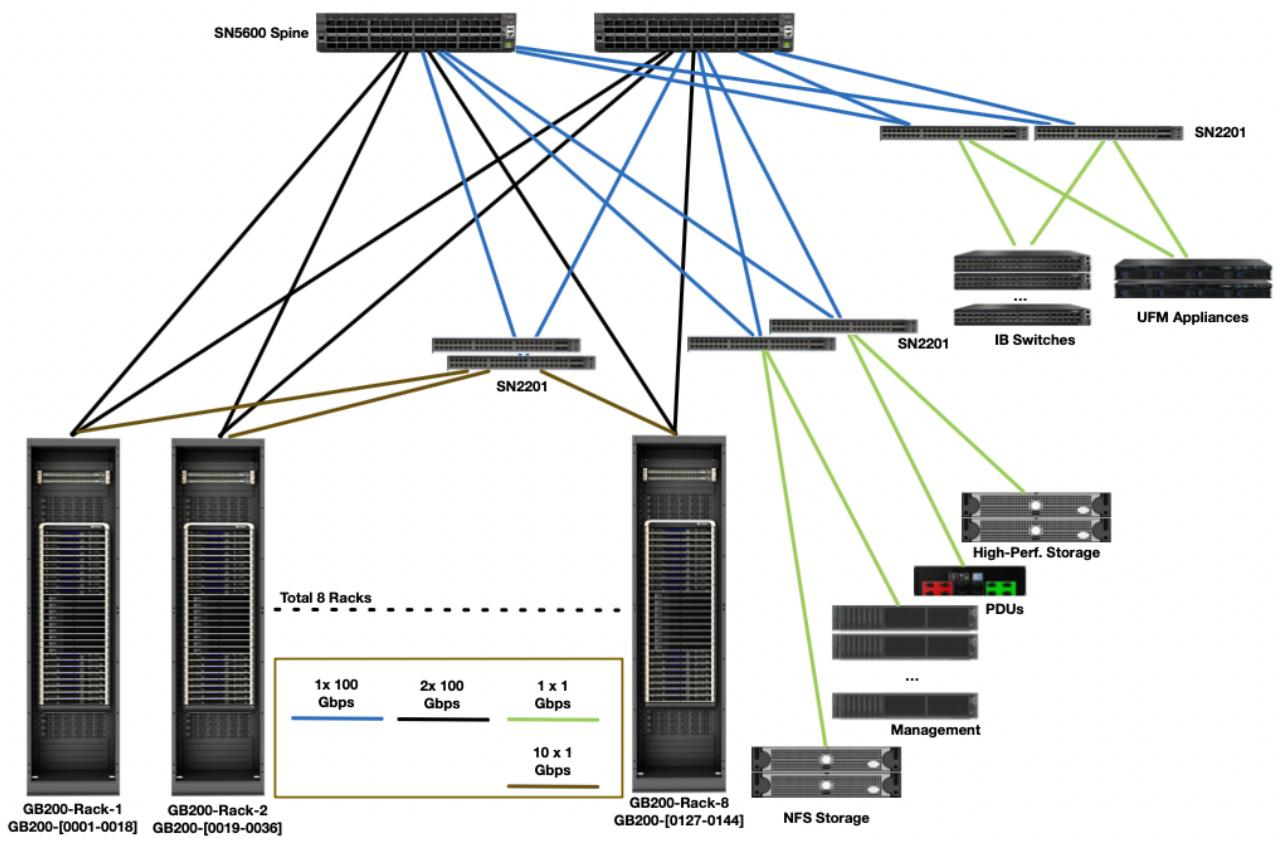
\includegraphics[keepaspectratio,alt={image}]{images/16bea45b9452267f759964b9f30f63da6ad598d13d012ddfcbfdc76d712d9865.jpg}}

Figure 4.10: Logical OOB management network layout

\pandocbounded{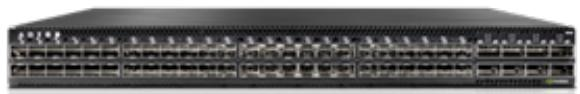
\includegraphics[keepaspectratio,alt={image}]{images/e5367555bf80199b66aa8c36c07a636e408faee104dd23673fc466b516422cfd.jpg}}

Figure 4.11: SN2201 switch

\section{4.5. Customer Edge
Connectivity}\label{customer-edge-connectivity}

For connecting DGX SuperPOD to customer edge for uplink and customer
corporate network access, we recommend at least 2x 100GbE links with DR1
single-mode connectivity to cope with the growing demand on high-speed
data transfer into and from DGX SuperPOD.

A new introduction to DGX SuperPOD with DGX GB200 systems because of its
complex cooling and power requirement is the connection to the Building
Management System (BMS). The BMS serves is the management plane of the
operational technology (OT) side of the data center infrastructure.

For route handover, we prepare eBGP protocol to peer with customer's
network. Routes to/from inband, out-of-band, and building management
system are announced. Figure 4.12 shows an example for customer edge
connectivity.

\pandocbounded{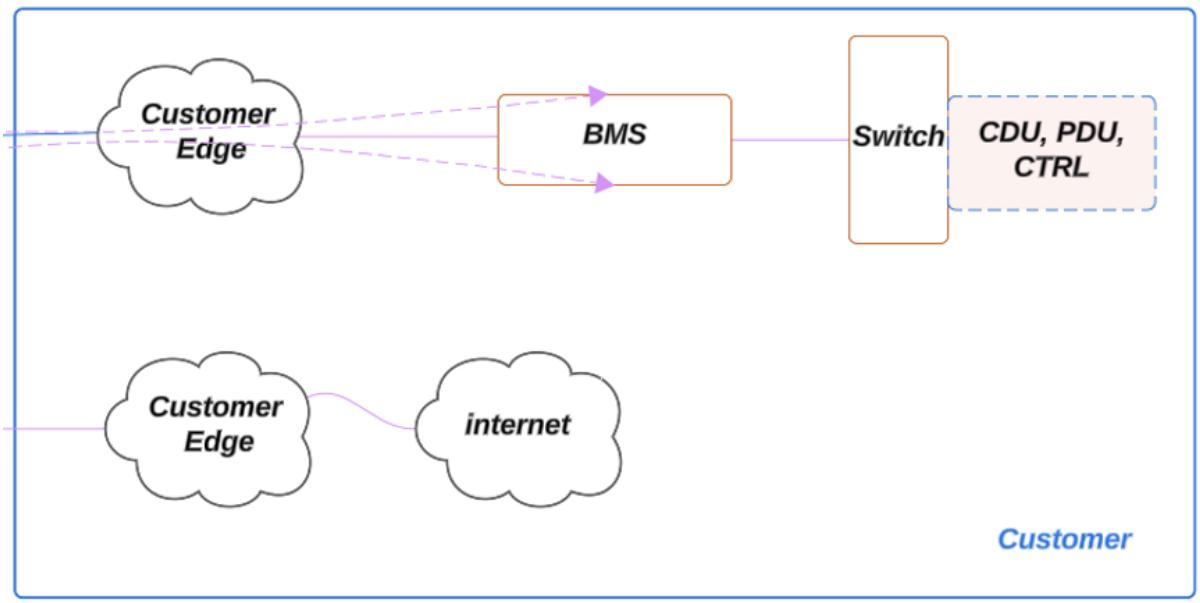
\includegraphics[keepaspectratio,alt={image}]{images/0d82310442100df3be03c61b64e287673edf524a4f004121b018b0626c466260.jpg}}

Figure 4.12: Example Customer Edge Connectivity

\section{Chapter 5. Storage
Architecture}\label{chapter-5.-storage-architecture}

Data, lots of data, is the key to development of accurate deep learning
(DL) models. Data volume continues to grow exponentially, and data used
to train individual models continues to grow as well. Data format, not
just volume can play a key factor in the rate at which data is accessed,
so storage system performance must scale commensurately.

The key I/O operation in DL training is re-read. It is not just that
data is read, but it must be reused again and again due to the iterative
nature of DL training. Pure read performance still is important as some
model types can train in a fraction of an epoch (ex: some recommender
models) and inference of existing can be highly I/O intensive, much more
so than training. Write performance can also be important. As DL models
grow and require more time to train, writing checkpoints is necessary
for fault tolerance. The size of checkpoint files can be terabytes in
size, and while not written frequently, are typically written in a
synchronously way that blocks forward progress of training process.

Ideally, data is cached during the first read of the dataset, so data
does not have to be repeatedly retrieved across the network. Shared
filesystems typically use RAM as the first layer of cache. Reading files
from cache can be an order of magnitude faster than from remote storage.
The DGX GB200 system provides local NVMe storage that can also be used
for caching or staging data.DGX GB200 systems provide local NVMe storage
that can also be used for caching or staging data.

DGX SuperPOD is designed to support all workloads, but the storage
performance required to maximize training performance can vary depending
on the type of model and dataset.

High-speed storage provides a shared view of an organization's data to
all nodes. It must be optimized for small, random I/O patterns, and
provide high peak node performance and high aggregate filesystem
performance to meet the variety of workloads an organization may
encounter. High-speed storage should support both efficient
multi-threaded reads and writes from a single system, but most DL
workloads will be read-dominant.Use cases in automotive and other
computer vision-related tasks, where high-resolution images are used for
training (and in some cases are uncompressed) involve datasets that
easily exceed 30 TB in size. In these cases, 4 GBps per GPU for read
performance is needed.

While NLP and LLM cases often do not require as much read performance
for training, peak performance for reads and writes are needed for
creating and reading checkpoint files. This is a synchronous operation,
and training stops during this phase. If you are looking for best
end-to-end training performance, do not ignore I/O operations for
checkpoints. Consider at least ½ of the read performance as recommended
write performance for LLM and large model use cases.

The preceding metrics assume a variety of workloads, datasets, and need
for training locally and directly from the high-speed storage system. It
is best to characterize workloads and organizational needs before
finalizing performance and capacity requirements. Table 5.1 and Table
5.2 are provided to help determine the I/O levels required for different
types of models.

Table 5.1: Storage Performance Requirements

{\def\LTcaptype{none} % do not increment counter
\begin{longtable}[]{@{}|l|l|l|@{}}
\toprule\noalign{}
\endhead
\bottomrule\noalign{}
\endlastfoot
\hline
Level & Work Description & Data Set Size \\
\hline
Standard & Multiple concurrent LLM or fine-tuning training jobs and
periodic checkpoints, where the compute requirements dominate the data
I/O requirements significantly. & Most datasets can fit within the local
compute systems\textquotesingle{} memory cache during training. The
datasets are single modality, and models have millions of parameters. \\
\hline
Enhanced & Multiple concurrent multimodal training jobs and periodic
checkpoints, where the data I/O performance is an important factor for
end-to-end training time. & Datasets are too large to fit into local
compute systems\textquotesingle{} memory cache requiring more I/O during
training, not enough to obviate the need for frequent I/O. The datasets
have multiple modalities and models have billions (or higher) of
parame-ters. \\
\hline
\end{longtable}
}

Table 5.2: Guidelines for storage performance

{\def\LTcaptype{none} % do not increment counter
\begin{longtable}[]{@{}|l|l|l|@{}}
\toprule\noalign{}
\endhead
\bottomrule\noalign{}
\endlastfoot
\hline
Performance Characteristic & Standard (GBps) & Enhanced (GBps) \\
\hline
Single SU aggregate system read & 40 & 125 \\
\hline
Single SU aggregate system write & 20 & 62 \\
\hline
4 SU aggregate system read & 160 & 500 \\
\hline
4 SU aggregate system write & 80 & 250 \\
\hline
\end{longtable}
}

\section{Chapter 6. DGX SuperPOD
Software}\label{chapter-6.-dgx-superpod-software}

NVIDIA Mission Control software delivers a full-stack data center
solution engineered for enterprise infrastructure deployments, like
NVIDIA DGX SuperPOD. It integrates essential management and operational
capabilities into a unified platform, providing enterprise customers
with seamless control over their infrastructure deployments at scale.

Figure 6.1 shows the detailed decomposition of DGX GB200 SuperPOD
software stack.

\pandocbounded{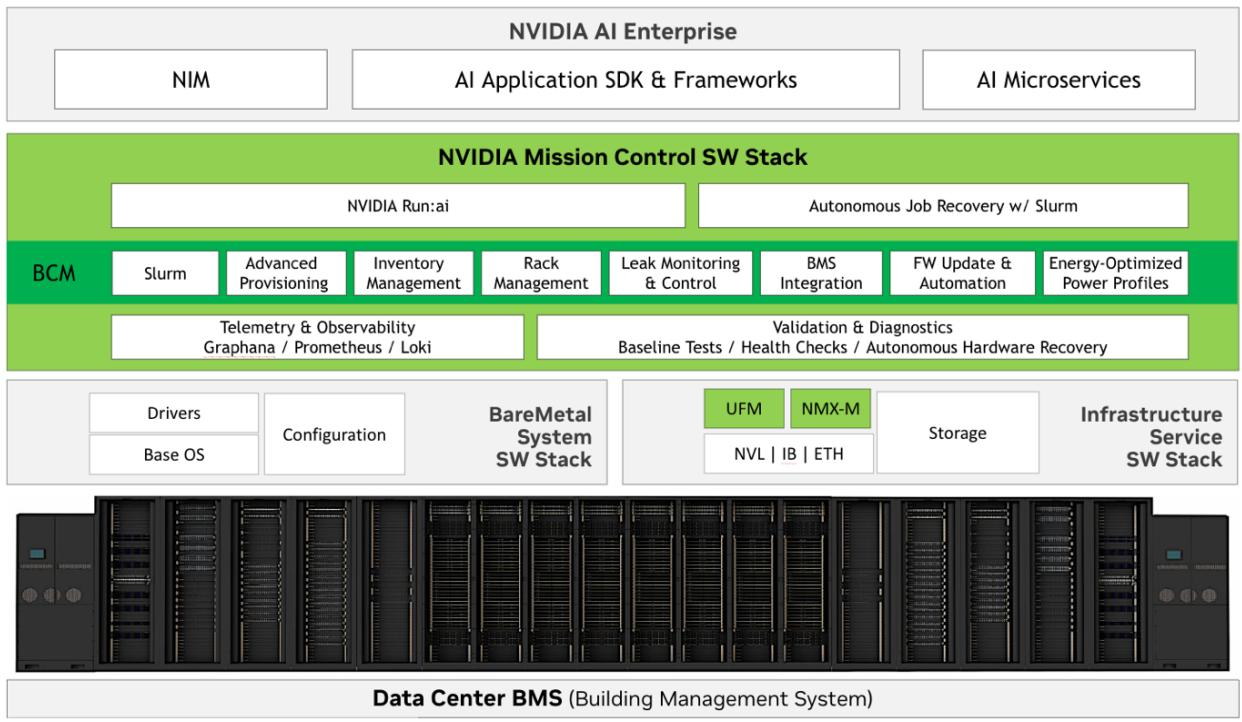
\includegraphics[keepaspectratio,alt={image}]{images/ba1ed79f5a9846920ca96d94f42b6ff3b4146113788c09d9f32d948ba380e074.jpg}}

Figure 6.1: NVIDIA DGX GB200 SuperPOD Software Stack

NVIDIA Mission Control software stack comprises a five-layer
architecture that builds from foundational system health and diagnostics
to advanced NVIDIA DGX SuperPOD cluster management operations. It
leverages NVIDIA Base Command Manager (BCM) technology and NVIDIA Run:ai
functionality to provide scheduler access with SLURM and Kubernetes for
AI and HPC workload orchestration. The Telemetry and Observability layer
leverages proprietary diagnostic tools and health-checks for system
insights, while the Validation and Diagnostics layer, supports the
built-in autonomous recovery engine that ensures rapid failure recovery
and system restoration with minimal time to recovery.

NVIDIA Mission Control also handles deployment optimization and system
health monitoring, seamlessly cooperating NVIDIA Base Command Manager
(BCM) technology for coordinating cluster provi-

sioning \& operations. Included in the software stack there is also
Network Management eXpert (NMX) for monitoring \& control of NVLINK
Switch trays.

NVIDIA Mission Control delivers critical innovations that directly
impact DL and HPC environments, improving efficiency, reducing downtime,
and optimizing resource utilization. Here's how these advancements
translate into tangible business value:

▶ Automated Failure Detection \& Self-Recovery: NVIDIA Mission Control's
automated failure detection and recovery mechanisms significantly
minimize downtime compared to manual interventions. With faster recovery
times, AI training continues without significant disruption, resulting
in improved GPU utilization. This reduces the risk of resource wastage.

▶ Optimized Workload Migration \& Resource Allocation: NVIDIA Mission
Control ensures that workloads are continuously reassigned to healthy
nodes, preventing idle GPU time. This leads to increased overall GPU
efficiency, enabling the system to process more workloads within the
same timeframe. By optimizing resource allocation, NVIDIA Mission
Control helps organizations achieve higher throughput for AI training
tasks, thereby accelerating time-to-results.

▶ Unified Diagnostics for Infrastructure \& Applications: By combining
infrastructure and application-level diagnostics, NVIDIA Mission Control
helps significantly reduce troubleshooting time. Model builders can
identify and resolve issues much faster compared to traditional methods.
This considerably decreases the operational burden on SREs and DevOps,
leading to savings in personnel costs and reducing the time to
production.

▶ In-Memory Checkpointing for Seamless Job Recovery: NVIDIA Mission
Control enables recovery of training workloads by automatically
restarting failed processes/ranks from the most recent valid checkpoint,
ensuring no data loss or rework. In environments with frequent failures,
it significantly reduces retraining time, thereby eliminating downtime
and preventing interruptions in the training loop. This results in an
increase in model iteration speed and faster go-to-market timelines for
AI products.

\section{6.1. Run:ai}\label{runai}

Included with NVIDIA Mission Control, the Run:ai platform employs a
distributed architecture consisting of two primary components: the
control plane (backend) and the cluster. The control plane serves as the
central management system, capable of orchestrating multiple Run:ai
clusters across an organization. For BCM-managed installations, the
control plane is hosted on the control plane while cluster components
are deployed directly onto the customer's Kubernetes infrastructure.
This separation of responsibilities allows for centralized management
while maintaining workload execution close to computational resources.

Figure 6.2 showcases the architecture of NVIDIA Run:ai

\pandocbounded{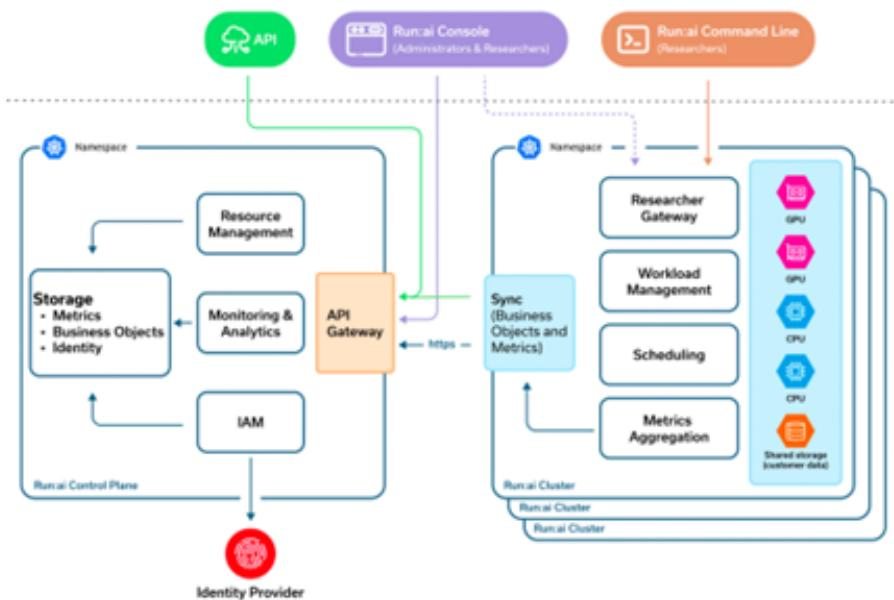
\includegraphics[keepaspectratio,alt={image}]{images/63d9e6477c5ec00630f1c36c4b8213c06ee53d73eeadc540a52a705296434a7f.jpg}}

Figure 6.2: NVIDIA Run:ai

\section{Chapter 7. Summary}\label{chapter-7.-summary}

NVIDIA DGX SuperPOD with NVIDIA DGX GB200 systems is the next generation
of data center scale architecture to meet the demanding and growing
needs of AI training and inferencing. This reference architecture
document for DGX SuperPOD represents the architecture used by NVIDIA for
our own AI model and HPC research and development. DGX SuperPOD
continues to build upon its highperformance roots to enable training of
the largest NLP models, support the expansive needs of training models
for automotive applications, and scaling-up recommender models for
greater accuracy and faster turn-around-time.

DGX SuperPOD represents a complete system of not just hardware but all
the necessary software to accelerate time-to-deployment, streamline
system management, proactively identify system issues. The combination
of all these components keeps systems running reliably, with maximum
performance, and enables users to push the bounds of state-of-the-art.
The platform is designed to both support the workloads of today and grow
to support tomorrow's applications. These are representatives of the
configuration and must be finalized based on actual design. Your NVIDIA
representative can work with you to finalize the exact components list.

\section{Chapter 8. Notices}\label{chapter-8.-notices}

\section{8.1. Notice}\label{notice}

This document is provided for information purposes only and shall not be
regarded as a warranty of a certain functionality, condition, or quality
of a product. NVIDIA Corporation (``NVIDIA'') makes no representations
or warranties, expressed or implied, as to the accuracy or completeness
of the information contained in this document and assumes no
responsibility for any errors contained herein. NVIDIA shall have no
liability for the consequences or use of such information or for any
infringement of patents or other rights of third parties that may result
from its use. This document is not a commitment to develop, release, or
deliver any Material (defined below), code, or functionality.

NVIDIA reserves the right to make corrections, modifications,
enhancements, improvements, and any other changes to this document, at
any time without notice.

Customer should obtain the latest relevant information before placing
orders and should verify that such information is current and complete.

NVIDIA products are sold subject to the NVIDIA standard terms and
conditions of sale supplied at the time of order acknowledgement, unless
otherwise agreed in an individual sales agreement signed by authorized
representatives of NVIDIA and customer (``Terms of Sale''). NVIDIA
hereby expressly objects to applying any customer general terms and
conditions with regards to the purchase of the NVIDIA product referenced
in this document. No contractual obligations are formed either directly
or indirectly by this document.

NVIDIA makes no representation or warranty that products based on this
document will be suitable for any specified use. Testing of all
parameters of each product is not necessarily performed by NVIDIA. It is
customer's sole responsibility to evaluate and determine the
applicability of any information contained in this document, ensure the
product is suitable and fit for the application planned by customer, and
perform the necessary testing for the application to avoid a default of
the application or the product. Weaknesses in customer's product designs
may affect the quality and reliability of the NVIDIA product and may
result in additional or different conditions and/or requirements beyond
those contained in this document. NVIDIA accepts no liability related to
any default, damage, costs, or problem which may be based on or
attributable to: (i) the use of the NVIDIA product in any manner that is
contrary to this document or (ii) customer product designs.

No license, either expressed or implied, is granted under any NVIDIA
patent right, copyright, or other NVIDIA intellectual property right
under this document. Information published by NVIDIA regarding
third-party products or services does not constitute a license from
NVIDIA to use such products or services or a warranty or endorsement
thereof. Use of such information may require a license from a third
party under the patents or other intellectual property rights of the
third party, or a license from NVIDIA under the patents or other
intellectual property rights of NVIDIA.

Reproduction of information in this document is permissible only if
approved in advance by NVIDIA in writing, reproduced without alteration
and in full compliance with all applicable export laws and

regulations, and accompanied by all associated conditions, limitations,
and notices.

THIS DOCUMENT AND ALL NVIDIA DESIGN SPECIFICATIONS, REFERENCE BOARDS,
FILES, DRAWINGS, DIAGNOSTICS, LISTS, AND OTHER DOCUMENTS (TOGETHER AND
SEPARATELY, ``MATERIALS'') ARE BEING PROVIDED ``AS IS.'' NVIDIA MAKES NO
WARRANTIES, EXPRESSED, IMPLIED, STATUTORY, OR OTHERWISE WITH RESPECT TO
THE MATERIALS, AND EXPRESSLY DISCLAIMS ALL IMPLIED WAR-RANTIES OF
NONINFRINGEMENT, MERCHANTABILITY, AND FITNESS FOR A PARTICULAR PURPOSE.
TO THE EXTENT NOT PROHIBITED BY LAW, IN NO EVENT WILL NVIDIA BE LIABLE
FOR ANY DAMAGES, INCLUDING WITHOUT LIMITATION ANY DIRECT, INDIRECT,
SPECIAL, INCIDENTAL, PUNITIVE, OR CON-SEQUENTIAL DAMAGES, HOWEVER CAUSED
AND REGARDLESS OF THE THEORY OF LIABILITY, ARIS-ING OUT OF ANY USE OF
THIS DOCUMENT, EVEN IF NVIDIA HAS BEEN ADVISED OF THE POSSIBILITY OF
SUCH DAMAGES. Notwithstanding any damages that customer might incur for
any reason whatsoever, NVIDIA's aggregate and cumulative liability
towards customer for the products described herein shall be limited in
accordance with the Terms of Sale for the product.

\section{8.2. Trademarks}\label{trademarks}

NVIDIA, the NVIDIA logo, NVIDIA DGX, and NVIDIA DGX SuperPOD are
trademarks and/or registered trademarks of NVIDIA Corporation in the
U.S. and other countries. Other company and product names may be
trademarks of the respective companies with which they are associated.

\section{8.3. Copyright}\label{copyright}

© 2024-2025, NVIDIA Corporation. All rights reserved.

\section{Copyright}\label{copyright-1}

©2024-2025, NVIDIA Corporation

\end{document}
